\documentclass[titlepage]{article}
\usepackage{graphicx}
\usepackage{multicol}
\usepackage[utf8]{inputenc}
\usepackage{authblk}
\usepackage{verbatim}
\usepackage{blindtext}
\usepackage[usenames]{color}
\usepackage{hyperref}
\usepackage[a4paper, margin=3cm]{geometry}

\usepackage[bottom]{footmisc}
\usepackage{float} % To place figures where I want them to be (with [H] option).
\usepackage{csquotes}
\usepackage{cancel}
\setlength{\parskip}{10px}

\usepackage{enumitem}
\usepackage{amsmath} %for using eqref
\usepackage{amssymb}
\usepackage{subfiles}

\usepackage[backend=biber, style=apa]{biblatex}
\addbibresource{bibliography.bib}
\usepackage{booktabs}
\usepackage{layouts}
\usepackage{dcolumn}
\usepackage{caption}
\usepackage{subcaption}

\usepackage{amsmath}
\usepackage[english]{babel}
\usepackage{amsthm}
\DeclareUnicodeCharacter{2212}{-}

\theoremstyle{plain}
\newtheorem{theorem}{Theorem}

\theoremstyle{plain}
\newtheorem{assumption}{Assumption}

\newtheorem*{assumptioncanonical}{Assumption (Canonical)}

\begin{document}

\title{Causal Inference - Replication Study}


\author[1]{Felipe Montealegre - 1035930}

\affil[1]{Alma Mater Studiorum - Università di Bologna}

\date{April 2023}

\maketitle


%%%%%%%%%%%%%%%%%%%%%%%%%%%%%%%%%%%%%%%%%%%%%%%%%%%%%%%%%%%%%%%%%%%%%%%%%%%
\section*{Overview and Guidelines for Replicating the Replication\footnote{Disclaimer: This is a replication exercise of Bansak and coauthors’ study on migrants' deaths and apprehensions in the US-Mexico border (\cite{Bansak2022}). Any mistakes are my own. For an accurate understanding of their study, please refer to the original article.}}

The following document contains a replication of \cite{Bansak2022} article (from now on referred to as BBC) as well as an extension. BBC uses a Differences in Differences (DiD) strategy to identify the causal effect of building fences on the US-Mexico border on the number of apprehensions and deaths. The extension is build on a more granular version of the original data set allowing for the identification of ATT type parameters across different doses. The extension includes replicating the same analysis of BBC and performing an event study to identify treatment effect dynamics across time. Additionally, it includes a skimming on the theory in \cite{callaway2021differenceindifferences} behind the identification of different parameters in a DiD setting, the estimation of ATTs for different dosis and the interpretation of the typical estimate obtained from a TWFE regression under the setting of multi-valued treatments.

This document is accompanied with a replication package for the replication study itself. It contains three main sub-folders and a readme file: \textit{\_draft}, that has the \LaTeX code for compiling this very same document, a \textit{\_replication} folder with the BBC original files and the \textit{.do} file used for replicating them, and a \textit{\_extention} folder with everything that is required for replicating the extension. The replication package can be downloaded from \href[]{https://github.com/felmola/_did_us_mexico_border.git}{https://github.com/felmola/\_did\_us\_mexico\_border.git}

\section*{Replicating \cite{Bansak2022}}

\subsection*{Technical details}

\begin{itemize}
    \item \textbf{Link to article:} \href{https://www.aeaweb.org/articles?id=10.1257/pandp.20221023}{https://www.aeaweb.org/articles?id=10.1257/pandp.20221023}.
    \item \textbf{Link to dataset and code:}\\
     \href{https://www.openicpsr.org/openicpsr/project/160201/version/V1/view}{https://www.openicpsr.org/openicpsr/project/160201/version/V1/view}.
    \item \textbf{Data and code availability:} Data and code are available for the replication study.
    \item \textbf{Code language:} STATA.
\end{itemize}

\subsection*{Context}

Donald Trump’s discurses for running for president of the USA for the 2017 – 2021 term revolved around a sound anti-immigration discourse , reviving strong nationalist feelings. In his discourse, one of the key promises was to deport all illegal immigrants and building a wall in the US-mexico border with the goal of stopping illegal migration, human trafficking, drug trafficking along the border, and protecting fellow Americans from border-related violence.

Advocacy for increasing border fencing is not a new idea. In 2006 President George W. Bush Signed the Secure Fence Act (SFA) that authorized the construction of hundreds of miles of new fencing under the same premise as Donald Trump.
While the potential benefits from building more fence around the border are intuitive, evidence shows that the real impact it has on immigration numbers and deaths across the border is null. The Government Acountability Office and literature explains that migrants simply walk around the fence or pass over it.


\subsection*{The Research Question}

The purpose of \cite{Bansak2022} article is to study the effect of building more fence on migrant flows and deaths. By exploiting data from the US Customs and Border Protection on apprehensions, deaths, staffing level, and border fencing compiled by Leo Castañeda and team (\cite*{castaneda2017}), they examine the effect of border fencing as a result of the SFA on migrants apprehensions and deaths at the border.

\subsection*{The Data}

There are 9 border sectors\footnote{From west to east along the border: San Diego, El Centro, Yuma, Tucson, El Paso, Big Bend, Del Rio, Laredo, Rio Grande Valley (See figure \ref{fig:border_sectors}). } along the US-Mexico border, and each of them is responsible for patrolling a continuous segment of the 1954 miles (3145 km) of its total extension. Each sector reports, year by year, from 1992 to 2019, the number of apprehensions and deaths from illegal migrants in the border (See figure \ref{fig:plot_cum_app} for a visualization of the number of apprehensions). The author include as covariates the number of months a sector had average temperatures above $80^{\circ}$ Fahrenheit and the number of border patrol staffing for each sector by year.

\begin{figure}[H]
\centering
    \caption{Cumulative apprehensions (millions) by sector across years.} 
    \label{fig:plot_cum_app} 
    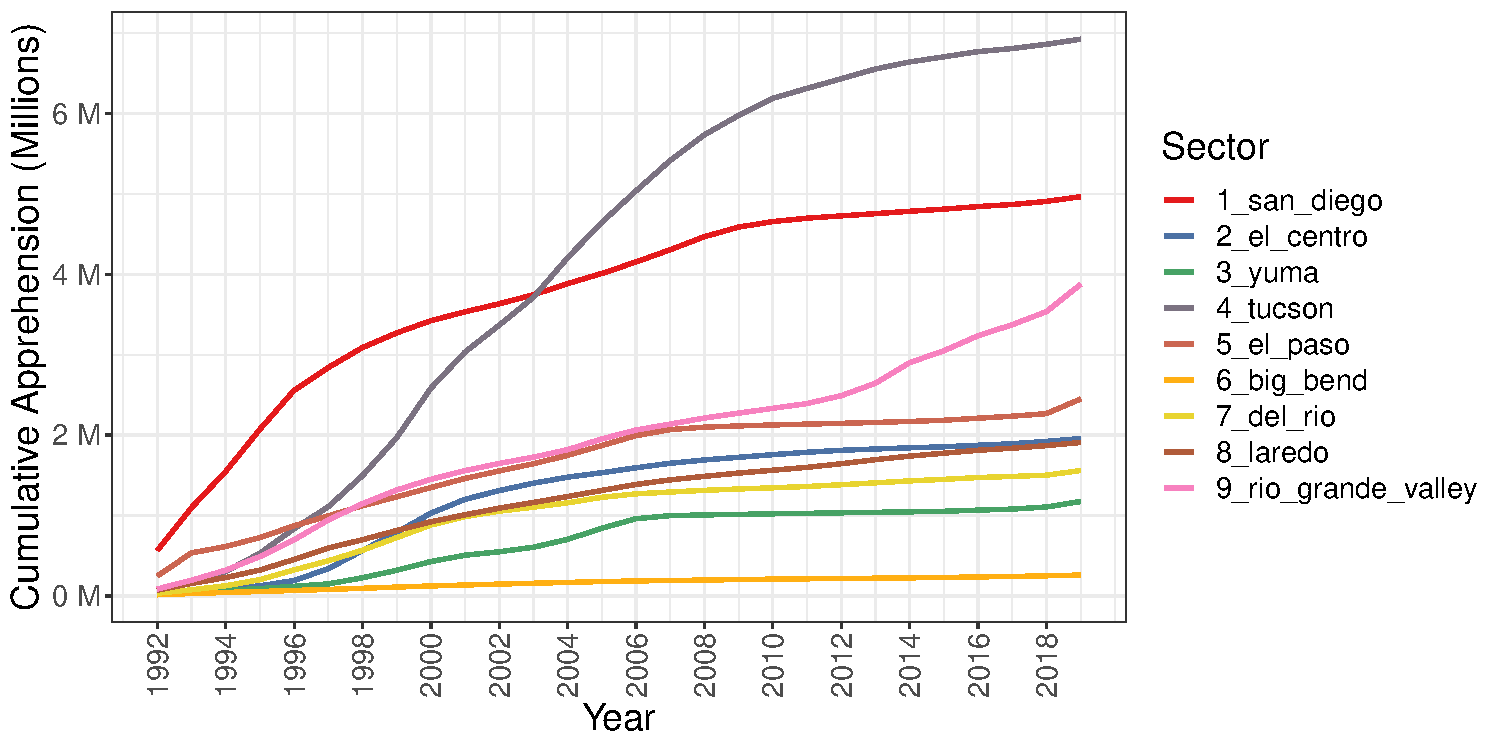
\includegraphics[width=\textwidth]{_images/plot_cum_app.pdf}
\end{figure}\textsc{}

\subsection*{Identification Strategy}

\subsubsection*{Potential Outcomes}

Let's introduce the following notation to avoid convoluted equations. Let $Y_{i,d,t}(d)$ be the potential outcome of unit $i$ at period $t$ had it been treated with dose $d$. In the canonical DiD, $d \in D=\{0,1\}$, and $t \in T=\{0,1\}$. $D$ is an indicator equal to 1 for sectors constructing new fencing after passing the SFA (i.e., the treatment group indicator) and 0 otherwise, $T$ is an indicator equal to 1 in the years after passing the SFA (i.e., the pre-post treatment indicator) and 0 otherwise. The parameter of interest is the Average Treatment Effect on the Treated (ATT), that is, the impact of fence construction, and is defined as follows:

\begin{equation}
\label{eq:att_1}
\begin{split}
	\textit{ATT} &= E[Y_{i,d,t}(1)|D=1,T=1] - E[Y_{i,d,t}(0)|D=1,T=1]\\
	&= E[\Delta Y_{i,d,t}|D=1] - E[\Delta Y_{i,d,t}|D=0]
\end{split}
\end{equation}

The second equality follows from applying \textit{SUTVA}, \textit{no anticipation}, and \textit{parallel trends} assumptions. Refer to annex \ref{appendix:canonical_derivation} for a detailed derivation.

\subsubsection*{Checking the Assumptions}

The authors indicate Yuma, Tucson, El Paso, San Diego, El Centro, and Rio Grande Valley, as the treated states. The control states are Big Bend, Del Rio, and Laredo. The authors define treatment assignment on the ground of being the states where \textit{most} of the new fencing was built \footnote{This treatment assignment scheme is challenged in the extension part of the study and provides the grounds for applying recent advances in the DiD literature.}. Only observations from 1998 to 2017 are included in the analysis. Years 2006 to 2008 are excluded from the analyses as fence built might be incomplete. No anticipation effects are assumed. Wall location is assumed to be exogenous (depends on environmental considerations rather than on the dependent variables).

The author assumes no anticipation effects thought one could argue that decisions of this magnitude are hard to keep hidden from, for example, border sector directives. If of public knowdledge they might reallocate resources or adopt policies due to the expectation of changes in the fencing composition along the border they protect. The author also assumes that the location of the wall is \enquote{plausibly exogenous} since fence location depends on environmental factors such as terrain, environmental impacts, land acquisitions, etc. One could argue that this might not be entirely true as sectors with higher number of illegal crossings could be specifically targeted for fence building, thus making the regressor endogenous. In one of the specifications, the authors include time-fixed effects to control for time trends affecting all sectors homogeneously.


\subsubsection*{Estimation Strategy}

The authors use the following TWFE model to estimate the ATT:

\begin{equation}
	\label{eq:twfe_1}
    Y_{idt} = \alpha + \beta_{1}\textit{D}_{d} + \beta_{2}\textit{T}_{t} + \theta(\textit{D}_{d} \times \textit{T}_{t}) + \Gamma X_{idt} + \epsilon_{idt},
\end{equation}

\noindent where $i$ is the border sector, $d$ is the treatment group, and $t$ is the pre-post treatment period. $Y_{idt}$ represents one of two outcome variables: either the natural logarithm of the number of apprehensions at the border, or the ratio $(\textit{Deaths}_{it}/\textit{Apprehensions}_{it} \times 100.000)$. As before, $D$ is an indicator equal to 1 for sectors constructing new fencing after passing the SFA (i.e., the treatment group indicator) and 0 otherwise, $T$ is an indicator equal to 1 in the years after passing the SFA (i.e., the pre-post treatment indicator) and 0 otherwise. $X_{it}$ is a vector of covariates including the lagged number of border patrol staff and the number of months when the temperature was above $80^{\circ}$ Fahrenheit. In a second specification, the authors include year fixed effects.

The link between the population parameters in the DiD strategy in equation \ref{eq:att_1} and the sample parameters in the TWFE estimation strategy in equation \ref{eq:twfe_1} is straightforward:

\begin{align}
\label{eq:parameters_1}
	\alpha &= E[Y_{i,d,t}|D=0,T=0]\\
	\beta_{1} &= E[Y_{i,d,t}|D=1,T=0] - E[Y_{i,d,t}|D=0,T=0]\\
	\beta_{2} &= E[Y_{i,d,t}|D=0,T=1] - E[Y_{i,d,t}|D=0,T=0]\\
	\theta &= (E[Y_{i,d,t}|D=1,T=1]-E[Y_{i,d,t}|D=1,T=0])-(E[Y_{i,d,t}|D=0,T=1]-E[Y_{i,d,t}|D=0,T=0])
\end{align}

%E[Y_{i,d,t}|D=x,T=x]

\subsection*{Replication and Results}

I used the replication package provided by the author containing the STATA code and the database used for the analysis contained in Table 1 of their article. All coefficients, p-values, standard errors, F-statistics, and the number of observations reported in the article match the ones obtained from running their replication package. Minor formatting issues were easily fixable. For example, the output from the replication package showed that the order of columns 3 and 4 were switched, year fixed effects dummies were included in the table, significance stars were also included. An attempt to replicate table 1 from their paper is shown in table \ref{tab:table1} below.

\begin{table}[htbp]\centering
\def\sym#1{\ifmmode^{#1}\else\(^{#1}\)\fi}
\caption{Estimation Results \label{tab:table1}}
\begin{tabular}{l*{4}{c}}
\hline\hline
            &\multicolumn{1}{c}{(1)}&\multicolumn{1}{c}{(2)}&\multicolumn{1}{c}{(3)}&\multicolumn{1}{c}{(4)}\\
            &\multicolumn{1}{c}{lnapp}&\multicolumn{1}{c}{lnapp\_c}&\multicolumn{1}{c}{deathsper100k}&\multicolumn{1}{c}{deathsper100k\_c}\\
\hline
fenced      &      1.1383\sym{***}&      0.6953\sym{***}&     -0.2904         &    -12.2415\sym{*}  \\
            &    (0.2222)         &    (0.1461)         &    (3.9056)         &    (5.1674)         \\
[1em]
sfa         &     -1.1029\sym{***}&     -2.2395\sym{***}&     82.6423\sym{***}&     85.6715\sym{**} \\
            &    (0.2654)         &    (0.2919)         &   (13.6249)         &   (30.3987)         \\
[1em]
fencedsfa   &     -0.4004         &     -0.8258\sym{***}&    -50.0210\sym{**} &    -63.5672\sym{***}\\
            &    (0.3176)         &    (0.1988)         &   (15.2819)         &   (13.4538)         \\
[1em]
months80    &                     &      0.1409\sym{***}&                     &      8.4761\sym{***}\\
            &                     &    (0.0313)         &                     &    (1.6433)         \\
[1em]
lagstaff    &                     &      0.0010\sym{***}&                     &      0.0294\sym{***}\\
            &                     &    (0.0001)         &                     &    (0.0055)         \\
[1em]
\_cons      &     10.7314\sym{***}&     10.2220\sym{***}&     28.7065\sym{***}&    -16.4512         \\
            &    (0.2030)         &    (0.2860)         &    (3.2511)         &    (9.6161)         \\
\hline
\(N\)       &         153         &         153         &         153         &         153         \\
time\_fe     &          No         &         Yes         &          No         &         Yes         \\
F           &     58.0701         &     30.9446         &     19.7457         &      8.1555         \\
p           &      0.0000         &      0.0000         &      0.0000         &      0.0000         \\
\hline\hline
\multicolumn{5}{l}{\footnotesize Standard errors in parentheses}\\
\multicolumn{5}{l}{\footnotesize \sym{*} \(p<0.05\), \sym{**} \(p<0.01\), \sym{***} \(p<0.001\)}\\
\end{tabular}
\end{table}


%textwidth in cm: \printinunitsof{cm}\prntlen{\textwidth}

Table \ref{tab:table1} reports the results of the TWFE model in equation \ref{eq:twfe_1}. In the notation used before, $\textit{fenced} \equiv D_{d}$, $\textit{sfa} \equiv T_{t}$, and $\textit{fencedsfa} \equiv D_{d} \times T_{t}$. In Columns (1) and (2) the outcome variable is the natural logarithm of the number of apprehensions. And in columns (3) and (4), the outcome variable is the ratio of deaths per 100.000 apprehensions. Columns (2) and (4) include the lag of border patrol staff, the number of months a sector had an average temperature above $80^{\circ}$ Fahrenheit, and year fixed-effects as controls.

In columns (1) and (2), the coefficient for \textit{fenced} is positive and statistically significant, meaning that prior to passing the SFA, the number of apprehensions in sectors that built fences was significantly higher than those who did not. The coefficient for \textit{sfa} in both columns is negative and statistically significant, indicating that the number of apprehensions after passing the SFA for sectors that did not build any fence decreased. The interaction term in column (1) is not statistically significant suggesting that there is no difference in the number of apprehensions after passing the SFA between states that built fence and those which did not. However, after adding controls, the coefficient is negative and statistically significant, indicating that sectors that build fence after passing the SFA had an even larger decrease in the number of apprehensions at the border.

In column (3), the coefficient for \textit{fenced} is negative but not statistically significant, suggesting that prior passing the SFA the number of deaths per 100.000 apprehensions was not statistically different between treated and untreated sectors. The coefficient for \textit{sfa} is positive and statistically significant, meaning that the number of deaths by 100.000 apprehensions was significantly higher after passing the SFA for sectors that did not build fence. The interaction term is negative and statistically significant, indicating that states that built fence saw an increase in the ratio of deaths by apprehensions after passing the SFA but a smaller one than those which did not. Similar results hold when including controls in column (4), however the coefficient for \textit{fenced} is now statistically significant, meaning that sectors that build fence would have lower deaths ratio than those that did not, before passing the SFA.

The coefficients for \textit{fencedsfa} in column (2) and \textit{sfa} in column (4) indicate that even though building fence decreased border apprehensions after passing the SFA (an indication of less border crossings), migrants preferred to cross on unfenced and potentially more dangerous sectors, raising the number of deaths.

%%%%%%%%%%%%%%%%%%%%%%%%%%%%%%%%%%%%%%%%%%%%%%%%%%%%%%%%%%%%%%%%%%%%%%%%%%%
\section*{Extending on \cite{Bansak2022}}

\subsection*{Granular Data on Fence Length}

Recall that in the replication section I said that the treatment assignment scheme would be challenged. If a dataset containing detailed information on how much fence was built and when it was built I could exploit this information to make a better assessment on the factibility of DiD their DiD identification strategy, fortunately, an article by Leo Castañeda and Jean Guerrero \cite*{castaneda2017} contains an interactive map containing, year by year, the length of fence and the geographical position of built fence segments across years.

I was able to access their \textit{Geodatabase} file containing a list of all the sections of vehicular barrier and pedestrian fence built from 1962 to 2015. The database identifies for each section the geographical position the segment was built at, the sector where it was built, the year it was built, and the type of fence used \footnote{There are two categories of fences: Pedestrian fence and vehicular barriers. And each of them is subdivided into primary, secondary, or tertiary depending on the existence of previously built fence and the difficulty of crossing over it. Primary fence makes up the bulk of the built fence.}. As BBC does, I added up all the types and categories of fence into a single type of fence. Merging this new data set with BBC data set I construct a panel of sectors, year by year, with the lenght of built fence, the number of apprehensions, the number of deaths, the number of border patrol staff, and the temperature above $80^{\circ}$ Fahrenheit.

Figure \ref{fig:plot_cum_length} gives a visual representation of the cumulative length of fence, year by year, for each of the sectors. The first thing that catches the eye is that if the treatment variable is defined as the cumulative length of fence built, then there is no longer a binary treatment; also, there is have a dose dimension to the treatment (which in this case is not constant in time), and a treatment timing component. For example, from the figure can be seen that Tucson only started building fences around 2005 and continued to do so until 2012, while El Paso first started building fences around 1995, stopped until 2005 where continued building fences until 2009, and then stop building fences altogether. Also, There are sectors that never build any fence, such as Laredo.

\begin{figure}[H]
	\centering
	\caption{Cumulative length (miles) of built fence by sector across years.} 
	\label{fig:plot_cum_length} 
	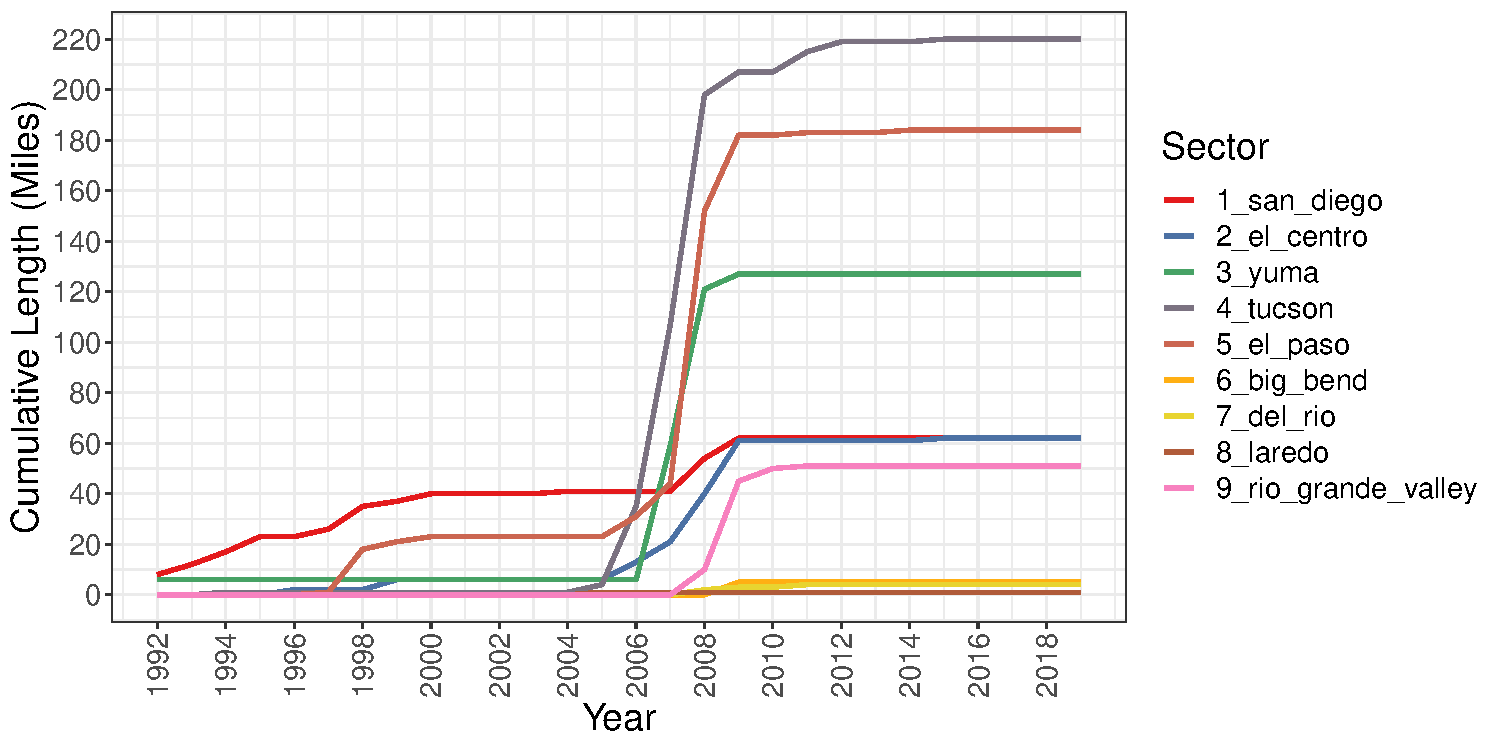
\includegraphics[width=\textwidth]{_images/plot_cum_length.pdf}
\end{figure}

Recent advances in the literature on DiD allows for both: different doses of treatment across groups (\cite{callaway2021differenceindifferences, chaisemartin2022}), differences in treatment timing (\cite{Callaway2021, GOODMANBACON2021254}) and even a combination of both (\cite{callaway2021differenceindifferences}). However, to the best of my knowledge, literature has not yet studied variations in treatment dosing within units. So, to comply with the setup of this literature, I must find a way to accommodate our data set.

When I compare our data set structure and the requirements from the current literature the data fails short to fulfill some of them. For instance, the first issue that I encounter is that the data set has units whose treatment status is non-zero pre-treatment, however, the literature requires that all units are untreated in the first time period. Big Bend, Del Rio, and Laredo had fence built pre-treatment, however the proportion of length of fence built to total length of the border sector is so minimal that I assume it is negligible. Therefore, I assume these sectors are the control group with no fence built pre-treatment period, as in the original paper. Nonetheless, San Diego and El Paso sectors had a non negligible length of fence built pre-treatment, and as such, they do not serve as good control groups so I drop them.

The second issue is that treatment status does not turn on like a switch. Fence building is a long process that requires time and effort to completion. As can be seen in figure \ref{fig:plot_cum_length}, sectors began building fence around 2005 and continue to do so until 2009. To comply with the recent literature where treatment status turns on or off (even if allowing for different doses) I drop observations from 2006 to 2009. Tucson sector continues to build a negligible amount of fence after 2009 so I standardize it to be constant across time. The resulting cumulative dose graph by sector across years is in figure \ref{fig:plot_dose}

I must also give compelling evidence that the common parallel trends assumption holds. Most macroeconomic shocks affect all sectors equally irrespective of their treatment status. Adding time trends allows to capture for this time fixed effects. However, Rio Grande Valley (RGV) apprehensions rates seem to behave contrary to what is expected. Upon closer examination, the dynamics of RGV are pretty peculiar. The increase in the number of apprehensions at this sector match an increase in the number of displaced families escaping to the USA through Mexico from gang violence in several Central American countries. The majority of this families opt for RGV and not other sectors because it is the closest one to the point of entry to Mexico. They choose so to reduce the costly and dangerous trip required to cross through farther away sectors. This shock that only affects RGV and that is not accounted for in the analysis would mean that RGV would have a different path in its potential outcome had it not built fence compared to the potential untreated outcomes of the other sectors, violating the parallel trends assumption. Therefore I drop it from the analysis.

After carefully selecting the control units and the treatment units and standardizing their treatment doses, the resulting cumulative length of fence by sector across years is reported in figure \ref{fig:plot_dose}. I end up with 3 control sectors (Big Bend, Del Rio, and Laredo) that are never treated, and 3 treated sectors that are treated with different doses of length of fence: El Centro, treated with 60 miles of fence, Yuma, treated with 130 miles of fence, and Tucson, treated with 220 miles of fence. This data set complies with the setting in \cite{callaway2021differenceindifferences}.

\begin{figure}[H]
	\centering
	\caption{Cumulative \enquote{dose} of fence by sector across years.} 
	\label{fig:plot_dose} 
	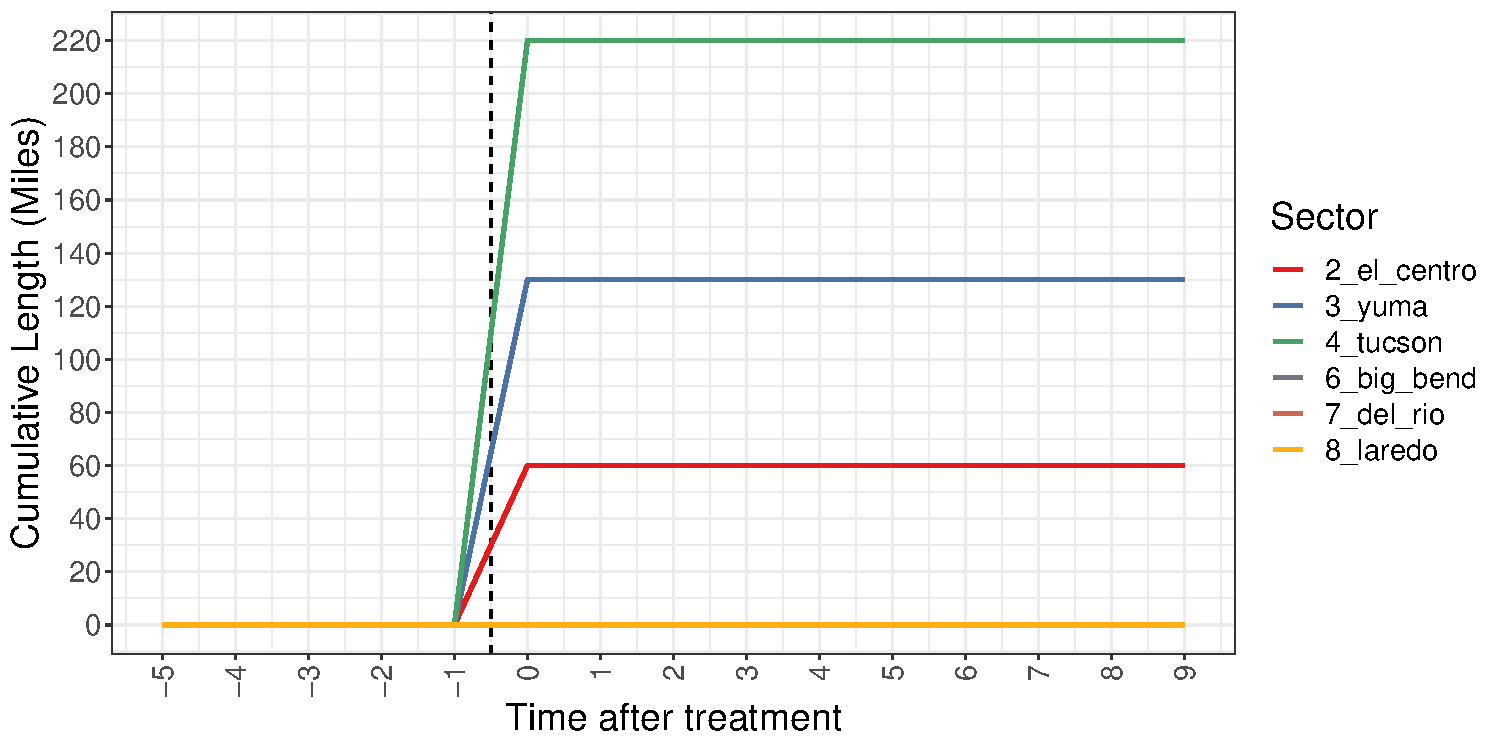
\includegraphics[width=\textwidth]{_images/plot_dose.pdf}
\end{figure}

\subsection*{Replicating BBC with the modified database}

Before moving forward with the advances in the DID literature, it is worth looking at BBC results with the modified data. To perform the same analysis, I define treatment status in the same spirit as the authors: the treatment indicator is a binary variable where El centro, Yuma, and Tucson are the treated units, and Big Bend, Del Rio, and Laredo serve as controls.

Table \ref{tab:table1_new} reports the regression results from the same specifications as in Table 1 from the original BBC article. In general, results go in the same direction.


\begin{table}
\caption{Replication results from Bansak et al. (2022) Table 1 with the new data set.}
\begin{center}
\begin{tabular}{l c c c c}
\hline
 & \multicolumn{2}{c}{ln(Apprehensions)} & \multicolumn{2}{c}{Death/Appehensions/100.000} \\
\cline{2-3} \cline{4-5}
 & (1) & (2) & (3) & (4) \\
\hline
treated       & $1.3187^{***}$  & $1.0700^{***}$  & $9.4282$        & $1.6066$         \\
              & $(0.3340)$      & $(0.2478)$      & $(5.2369)$      & $(9.0557)$       \\
post          & $-0.9665^{**}$  & $-0.7175$       & $86.0308^{***}$ & $47.0322^{*}$    \\
              & $(0.3008)$      & $(0.3862)$      & $(13.4450)$     & $(19.1518)$      \\
treated\_post & $-0.7952$       & $-1.1572^{***}$ & $-49.6933^{**}$ & $-69.8606^{***}$ \\
              & $(0.4173)$      & $(0.2903)$      & $(17.0428)$     & $(16.4691)$      \\
months80      &                 & $0.1705^{***}$  &                 & $11.7456^{**}$   \\
              &                 & $(0.0419)$      &                 & $(3.4085)$       \\
lag\_staff    &                 & $0.0009^{***}$  &                 & $0.0451^{***}$   \\
              &                 & $(0.0001)$      &                 & $(0.0065)$       \\
(intercept)   & $10.6531^{***}$ & $9.4109^{***}$  & $28.4529^{***}$ & $-39.9472^{*}$   \\
              & $(0.2531)$      & $(0.2647)$      & $(3.6250)$      & $(17.0688)$      \\
\hline
Fixed Effects & NO              & YES             & NO              & YES              \\
F             & $20.0358$       & $17.5443$       & $12.3329$       & $7.0746$         \\
Num. obs.     & $90$            & $78$            & $90$            & $78$             \\
\hline
\multicolumn{5}{l}{\scriptsize{$^{***}p<0.001$; $^{**}p<0.01$; $^{*}p<0.05$}}
\end{tabular}
\label{tab:table1_new}
\end{center}
\end{table}


\subsubsection*{Event Study}

The panel data structure of the data set is the perfect setting to set up an \enquote{event study}. Event studies allow for identification of dynamic treatment effects. The dynamics are captured by introducing leads and lags of the treatment variable in the standard TWFE setting in equation \ref{eq:twfe_1}. The new specification including treatment lead and lags is in equation \ref{eq:event_study} below.

\begin{equation}
	\label{eq:event_study}
	Y_{idt} = \alpha + \beta_{1}\textit{D}_{d} + \beta_{2}\textit{T}_{t} + \sum_{\tau = -p}^{-1}\theta_{\tau}(\textit{D}_{d} \times \textit{T}_{\tau}) + \sum_{\tau = 0}^{q}\theta_{\tau}(\textit{D}_{d} \times \textit{T}_{\tau})+ \Gamma X_{idt} + \epsilon_{idt},
\end{equation}

\noindent where $q$ is the number of periods the treatment is lagged, and $p$ is the number of leads. $\theta_{\tau}$ is their corresponding coefficients.

Equation \ref{eq:event_study} will output a coefficient for the treatment effect of the outcome variable for each of the time periods in the sample. Although not a test \textit{per se}, event studies could present a good case for the parallel trends assumption or can debunk it altogether. In principle, if PT holds, I would expect that the treatment coefficients in the years previous to passing the SFA would not be statistically different from zero since treatment exposure should not have any effect before treatment exposure. Furthermore, if the coefficients of the treatment become significant only after treatment exposure, it suggest that it is only through treatment exposure that these changes could take place. Figure \ref{fig:event_studies} displays the event study plots for the two outcome variables.

\begin{figure}
	\caption{Event study for the outcome variables.}
	\label{fig:event_studies}
	\centering
	\begin{subfigure}[b]{0.48\textwidth}
		\caption{Dynamic effects for ln(apprehensions).}
		\label{fig:es_app}
		\centering
		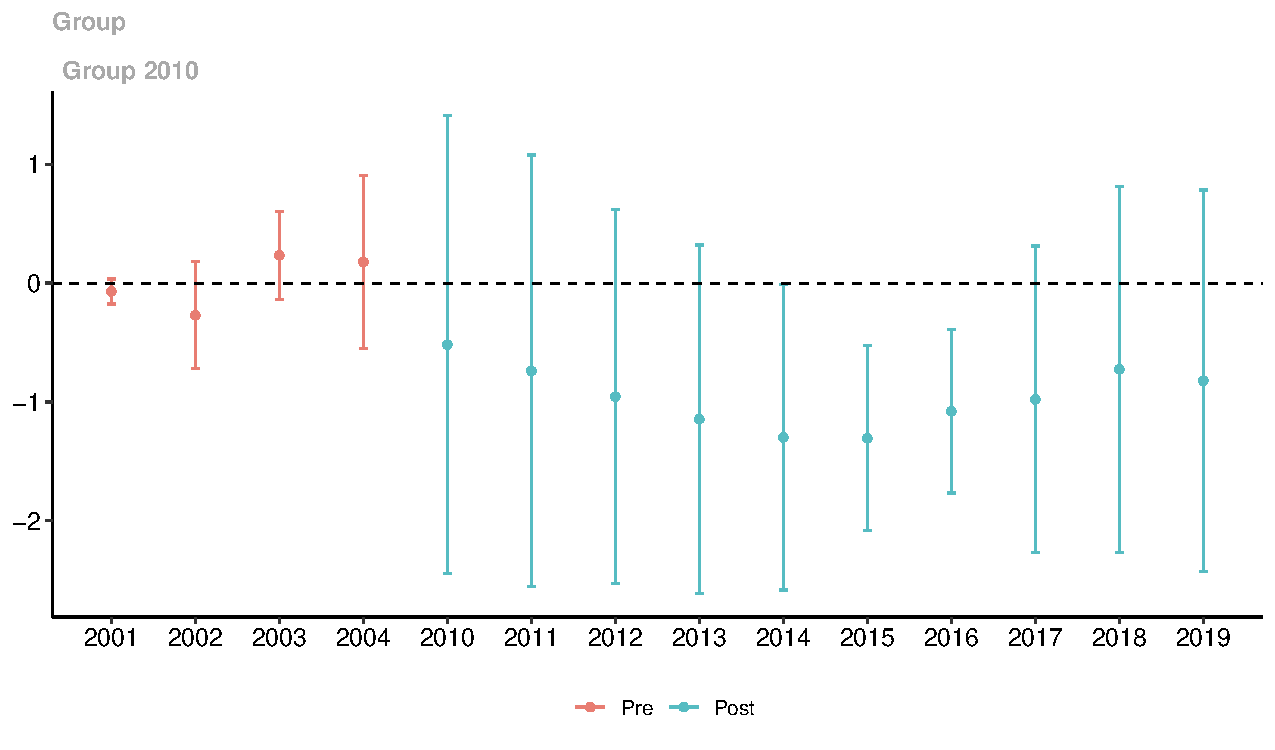
\includegraphics[width=\textwidth]{_images/plot_es_app.pdf}
	\end{subfigure}
	\begin{subfigure}[b]{0.48\textwidth}
		\caption{Dynamic effects for death ratio.}
		\label{fig:es_death}
		\centering
		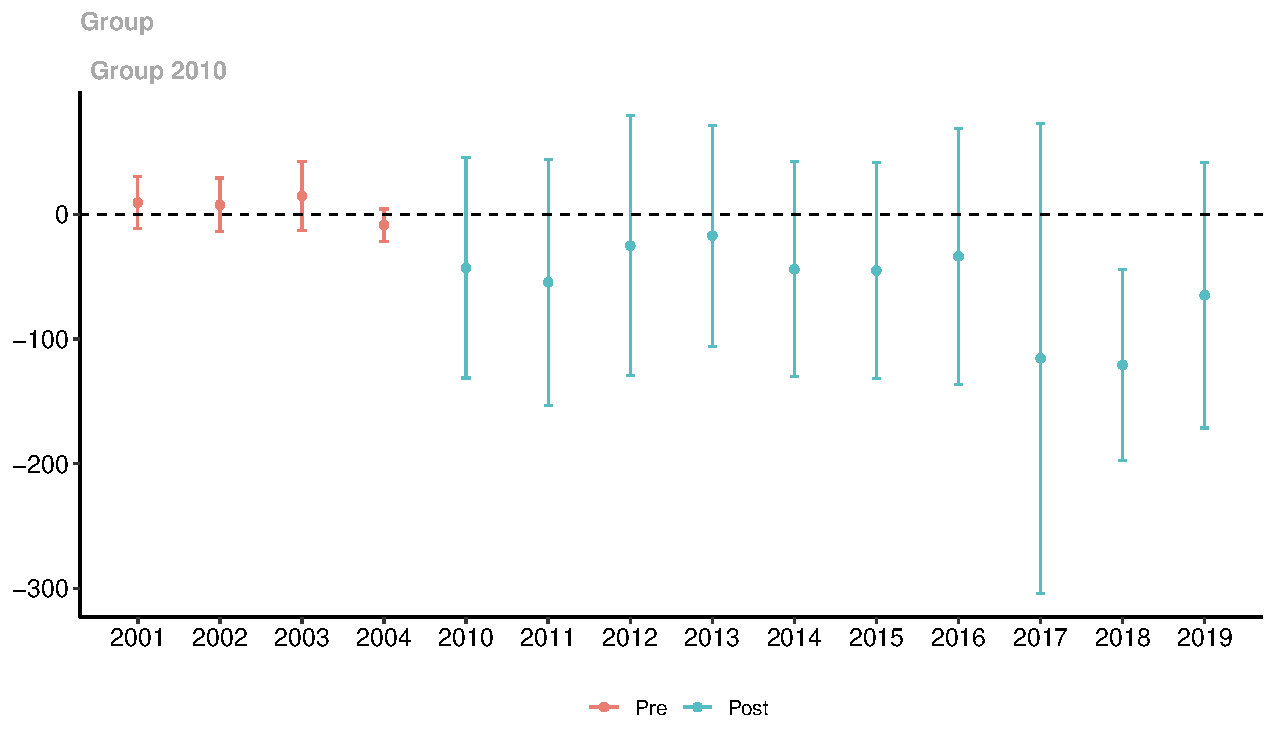
\includegraphics[width=\textwidth]{_images/plot_es_death.pdf}
	\end{subfigure}
\end{figure}

Figure \ref{fig:event_studies} tells an interesting story. For none of the two outcome variables do the coefficients’ confidence intervals exclude zero for the periods before treatment assignment. This indicates that building fence had no effect whatsoever on  neither the natural logarithm of apprehensions nor on the ratio of deaths per 100.000 apprehensions, before passing the SFA, convincing the reader that perhaps the PT assumption could hold in this setting. Even more, \ref{fig:es_app} shows treatment effect dynamics in the number of apprehensions: building fence has no immediate effect after building fence but has a delayed effect that starts 4 periods after treatment \footnote{The delay in treatment effect could be an artifact of small power due to the small sample size.}, and then the effect slowly fades out. This could obey to increasingly innovative ways in which carters and people smugglers cross the border and the use of technology to support people and drug smuggling.

Nonetheless, figure \ref{fig:es_death} shows not evidence supporting any effect of building fence after passing the SFA on the deaths ratio \footnote{With the exception of 2018. This fluke could be due to the small sample size as it is very unlikely that building fence has such a very specific dynamic-effect pattern.}. As in BBC, this is evidence that even though building fence after passing the SFA reduces apprehensions at the border, migrants are diverting towards unfenced and more dangerous crossing sites. 	 


\subsection*{DiD with Heterogeneity in Treatment Dose\footnote{This section draws heavily from \cite{callaway2021differenceindifferences}}}

Recall that figure \ref{fig:plot_dose} shows the (adjusted) cumulative length of fence built for every state across time. There are some sectors that never build fence and some others that build fence after passing the SFA, however they do so in different measures. Under this setting, the parameters of interest that can be estimated go beyond the ATT in the 2$\times$2 canonical DiD. Here I can obtain dose specific ATTs and even estimate a new type of parameter: the Average Causal Response (ACRT) of a higher dose compared to a lower one for those treated with the higher dose.
To estimate this kind of parameters, a common practice in the literature is to use a TWFE regression model as the one defined in equation \ref{eq:beta_12}. The only difference is that $D_{d}$ is allowed to take on values beyond 0 or 1. According to \cite{callaway2021differenceindifferences}, without making any assumptions beyond random sampling and assuming  that all units are not exposed to treatment in the first period, $\theta^{twfe}$ is defined as


\begin{flalign}
\label{eq:beta_12}
	\theta^{twfe} = \sum_{d_j \in \mathcal{D}_+} w_1(d_j) \frac{E[\Delta Y_t |D=d_j] - E[\Delta Y_t |D=d_{j-1}]}{d_j - d_{j-1}}
\end{flalign}

$\theta^{twfe}$ in \ref{eq:beta_12} is just the weighted average of differences the expectation function conditional on the dose and as such, there is not a direct mapping between this estimate and any causal parameter of interest.

\subsubsection*{The Theory}
	
What kind of parameters are interesting to estimate in a setting with multi-valued treatments? The multi-valued treatment setup allows to estimate level effects and slope effects or \enquote{causal responses}. The most common parameters to estimate in levels are the ATT($d|d$) and the ATE($d$):

\begin{flalign*}
\label{eq:att_ab}
	ATT(a|b)=\mathbb{E}[Y_{t}(a)-Y_{t}(0)|D=b] \textit{ and } ATE(d)=E[Y_{t}(d)-Y_{t}(0)].
\end{flalign*}

The ATT($a|b$) is the average effect of dose a on units exposed to dose b. In general, for this kind of analysis the ATT($d|d$) is a more interesting parameter to identify. The ATE($d$) is the average difference between potential outcomes of units treated with dose d relative to untreated treated over all units.

The common parameters to estimate in slope terms are the ACRT($d{j}|d_{j}$) and the ACR($d_{j}$):

\label{eq:acrt}
\begin{flalign*}
	ACRT(d_j|d_j)=E[Y_{t}(d_j)-Y_{t}(d_{j-1})|D=d_j] \textit{ and } ACR(d_j)=E[Y_{t}(d_j)-Y_{t}(d_{j-1})].
\end{flalign*}

The ACRT($d_{j}|d_{j}$) is the difference in potential outcomes between dose $d_{j}$ and the next lower dose for units actually treated with dose $d_{j}$. The ACR($d_{j})$ is the difference in potential outcomes between two adjacent doses for all the units. Notice that in the ATT would be equivalent to the ACRT if doses were adjacent to one another.

How are these parameters identified? \cite{callaway2021differenceindifferences} propose a set of assumptions that allow for the identification of these parameters:

\begin{assumption}[Random Sampling]
	\label{ass1}
	The observed data consists of  $\left\{Y_{it}, Y_{it-1}, D_i\right\}_{i=1}^n$ which is independent and identically distributed.
\end{assumption}

\begin{assumption}[Support (for Multi-valued treatments)]
	\label{assMV}
The support of $D, \mathcal{D} = \left\{0\right\} \cup \mathcal{D}_+$ where $\mathcal{D}_+ =
\left\{d_1, d_2, \textit{. . .} , d_J \right\}$ where $0 < d_1 < d_2 < \textit{. . .} < d_J$ . In addition, $P(D = d) > 0$ for all $d \in \mathcal{D}$.
\end{assumption}

\begin{assumption}[Observed Outcomes / No Anticipation]
	\label{ass3}
	For all units,
	\begin{equation*}
		Y_{it−1} = Y_{it−1}(0) \textit{ and } Y_{it} = Y_{it}(D_i).
	\end{equation*}
\end{assumption}

\begin{assumption}[Parallel Trends]
	\label{ass4}
	For all $d \in \mathcal{D}$,
	\begin{equation*}
		\mathbb{E}[Y_t(0)-Y_{t-1}(0)|D=d] = \mathbb{E}[Y_t(0)-Y_{t-1}(0)|D=0].
	\end{equation*}
\end{assumption}

\begin{assumption}[Strong Parallel Trends]
	\label{ass5}
	For all $d \in \mathcal{D}$,
	\begin{equation*}
		\mathbb{E}[Y_t(d)-Y_{t-1}(0)] = \mathbb{E}[Y_t(d)-Y_{t-1}(0)|D=d].
	\end{equation*}
\end{assumption}

Under Assumptions 1 to 4, $ATT(d|d)$ is identified for all $d \in \mathcal{D}$, and it is given by
\begin{equation*}
	ATT(d|d)= E[\Delta Y_t |D=d] - E[\Delta Y_t |D=0].
\end{equation*}

ATT is the average difference between the potential outcomes of being treated with dose $d$ with respect to not being treated, for those actually treated with dose $d$. This result exploits assumption 4 by assuming that in the absence of the dose, the difference in potential outcomes between units treated with dose $d$ and units never treated would have been the same.

While it is tempting to compare ATT($d|d$) for different doses $d$ as a causal effect of dose $d$ relative to some other dose $d’$ by computing the difference between them, even under assumptions 4 or 5, this difference is given by


\begin{flalign}
\label{eq:att_bias_1}
	ATT(d|d) - ATT(d'|d') = ATT(d|d) - ATT(d'|d)  +  \underbrace{ATT(d'|d) - ATT(d'|d')}_{ \textit{selection bias}}.
\end{flalign}

\noindent where the first term to on the RHS is the difference in the ATTs of being treated with dose $d$ with respect to being treated with dose $d’$, for those units actually treated with dose $d$ (i.e. a meaningful parameter to be estimated) the second term a selection bias associated to the differential effect that dose $d’$ has on units actually treated with $d´$ and with dose $d$.

Under Assumption 4, the selection bias is decomposed as

\label{eq:attdd2}
\begin{flalign*}
	ATT(d'|d) - ATT(d'|d')= E[Y_{t}(d')-Y_{t-1}(0)|D=d] - E[Y_{t}(d')-Y_{t-1}(0)|D=d'].
\end{flalign*}

\noindent where the second term on the RHS is the (observed) difference in the potential outcomes of units treated with dose $d'$ with respect to not being treated, for those units actually treated with dose $d'$. On the contrary, the second term is a counterfactual and cannot be obtained in the sample. However, Assumption 4 cannot be invoked on the first term because it says nothing about treated potential outcomes.

In terms of slopes and under the same assumptions, the result obtained from comparing ATTs for neighboring doses is decomposed as

\label{eq:prop3a}
\begin{flalign*}
	E[\Delta Y_t |D=d_j]-E[\Delta Y_t |D=d_{j-1}]= ACRT(d_j|d_j)+ \underbrace{ATT(d_{j-1}|d_j) - ATT(d_{j-1}|d_{j-1})}_{ \textit{selection bias}}
\end{flalign*}

The selection bias comes from the same source as in the levels case. It is the result of heterogeneous effects of dose $d'$ on units actually treated with dose $d$ and dose $d'$.

Under Assumptions 1 to 4 the estimate obtained from TWFE in equation \ref{eq:twfe_1} is 

\label{eq:beta_14}
\begin{flalign*}
	\theta^{twfe} = \sum_{d_j \in \mathcal{D}_+} w_1(d_j) \left(\frac{ACRT(d_j|d_j)}{d_j - d_{j-1}}+\frac{(ATT(d_{j-1}|d_j)-ATT(d_{j-1}|d_{j-1}))}{d_j - d_{j-1}}\right)
\end{flalign*}

This estimate is a weighted average of the ACRT for different doses and some selection bias terms as described before.

If assumption 4 gets replaced by the stronger Assumption 5, then the ACR($d_{j}$) is identified as

\label{eq:prop3b}
\begin{flalign*}
	E[\Delta Y_t |D=d_j]-E[\Delta Y_t |D=d_{j-1}]= ACR(d_j)
\end{flalign*}

Under assumption 5, 

\label{eq:beta_15}
\begin{flalign}
	\theta^{twfe} = \sum_{d_j \in \mathcal{D}_+} w_1(d_j) \frac{ACR(d_j)}{d_j - d_{j-1}}
\end{flalign}

\subsubsection*{Results}

Table \ref{tab:cw_atts} shows the calculated ATTs for each of the different doses. I will focus on columns (2) and (4) that, as in BBC article, includes the number of months where each state had temperatures above $80^{\circ}$ Fahrenheit, the lagged number of border patrol staff and time year fixed effects.


\begin{table}
\caption{TWFE estimation of ATTs across doses.}
\begin{center}
\begin{tabular}{l c c c c}
\hline
 & \multicolumn{2}{c}{ln(Apprehensions)} & \multicolumn{2}{c}{Death/Appehensions/100.000} \\
\cline{2-3} \cline{4-5}
 & (1) & (2) & (3) & (4) \\
\hline
treated d=60   & $1.0833^{**}$   & $1.0115^{***}$  & $23.4394^{***}$   & $-6.8694$        \\
               & $(0.3268)$      & $(0.2799)$      & $(6.8428)$        & $(21.0716)$      \\
treated d=130  & $0.5399$        & $1.0108^{**}$   & $5.6412$          & $-18.7532$       \\
               & $(0.3061)$      & $(0.3657)$      & $(4.2802)$        & $(24.7956)$      \\
treated d=220  & $2.3328^{***}$  & $0.9101$        & $-0.7958$         & $39.2162$        \\
               & $(0.2803)$      & $(0.7037)$      & $(6.4689)$        & $(47.6940)$      \\
post           & $-0.9665^{**}$  & $-0.9080^{**}$  & $86.0308^{***}$   & $52.9012^{*}$    \\
               & $(0.3081)$      & $(0.3178)$      & $(13.7691)$       & $(23.2524)$      \\
ATT(60$|$60)   & $-0.7711^{*}$   & $-0.4138$       & $-101.9182^{***}$ & $-97.2279^{***}$ \\
               & $(0.3837)$      & $(0.2276)$      & $(15.7358)$       & $(18.4148)$      \\
ATT(130$|$130) & $-0.9343^{*}$   & $-0.7810^{*}$   & $-66.8223^{**}$   & $-53.3093^{*}$   \\
               & $(0.4323)$      & $(0.3095)$      & $(19.7110)$       & $(22.8067)$      \\
ATT(220$|$220) & $-0.6802$       & $-3.3040^{***}$ & $19.6606$         & $-14.7934$       \\
               & $(0.3630)$      & $(0.7720)$      & $(17.5143)$       & $(47.9303)$      \\
months80       &                 & $0.0418$        &                   & $19.5970^{*}$    \\
               &                 & $(0.1165)$      &                   & $(8.7299)$       \\
lag\_staff     &                 & $0.0016^{***}$  &                   & $0.0204$         \\
               &                 & $(0.0004)$      &                   & $(0.0255)$       \\
(intercept)    & $10.6531^{***}$ & $9.2595^{***}$  & $28.4529^{***}$   & $-41.1435$       \\
               & $(0.2592)$      & $(0.2204)$      & $(3.7124)$        & $(20.7012)$      \\
\hline
Fixed Effects  & NO              & YES             & NO                & YES              \\
F              & $20.7296$       & $23.4513$       & $10.3070$         & $5.9073$         \\
Num. obs.      & $90$            & $78$            & $90$              & $78$             \\
\hline
\multicolumn{5}{l}{\scriptsize{$^{***}p<0.001$; $^{**}p<0.01$; $^{*}p<0.05$}}
\end{tabular}
\label{tab:cw_atts}
\end{center}
\end{table}


Table \ref{tab:cw_atts} tells an interesting story. The coefficients \textit{treated D=d} indicate that before passing the SFA, all sectors that build fence, irrespective of the length built, had a significantly higher number of apprehensions at the border when contrasted to sectors that did not build any fence. The coefficient \textit{post} says that sectors that never built fence had a decrease in the number of apprehensions after passing the SFA relative to the time before the SFA.

The different values for the ATTs across doses is an indicator of treatment heterogeneity across dose. For example, the average effect of building fences for those sectors that built 60 miles of fence (the lowest amount) is negative but not significantly different from the number of apprehensions in sectors that did not build fence before passing the SFA. However, the ATT for sectors building 130 miles of fence, the effect is not statistically different from the control sectors before passing the SFA, and larger in magnitude. The largest effect on the number of apprehensions for treated sectors after passing the SFA is for the sectors that build 220 miles of fence. These results suggest that there is an incremental effect of building miles of fence on the number of apprehensions in the border.

When looking at the \textit{treated D=d} coefficients on column (4) it can be seen before passing the SFA, irrespective of the \enquote{dose}, there was not any significant difference in the number of deaths at the border between sectors that built fence and those that did not. The \textit{post} coefficient shows that sectors that never build fence had higher deaths at the border after passing the SFA.

When looking at the ATTs across doses on the number of deaths, it can be seen that there is also treatment effect heterogeneity across dose. The most interesting part of this story is that between the sectors that built fence, the highest decrease in the number of deaths at the border is for those who did so in the least amount. Taken together, the new results weaken the story told in BBC. Under BBC, it is expected that sectors with greater lengths of fence would see the greates decreases in the number of deaths in the border, and those sectors with the least amounts of dence build (excludign zero-length sectors) would see the lowest decrease in the number of deaths. Nonetheless, as expected, the sectors that did not buuld fence saw the greatest increase in the number of deaths at the border.

Beware that the previous argument explicitly compares ATTs across does, however, recall from the discussion in \cite{callaway2021differenceindifferences} that not even that under the stronger Assumption 5 it is possible to get rid of the selection bias when comparing two different ATTs. The bias in equation \ref{eq:att_bias_1} requires that the differences in the potential outcomes had they been treated with dose $d'$ between sectors treated with dose $d$ and $d'$ would have been the same. This assumption is very likely to fail. For example, it can be argued that there might be environmental factors that could make the diference in the potential number of deaths for a sector had it built 130 miles of fence and the potential outcome had it build 220 miles of fence, of a sector that actually build 220 miles of fence, different from the same difference in potential outcomes but on a sector that build 130 miles of fence. Without a deeper understanding of the assignment process and of the environment, local and political dynamics of sector administration, it is not possible to defend comparisons between ATTs across doses.

Finally, I present the results of the TWFE regression model in equation \ref{eq:twfe_1} by building off of Assumption 5 so that $\theta^{twfe}$ can be interpreted as a weighted average of ACR for all doses if the weighted scheme is known by the researcher. Results are in table \ref{tab:cw_twfe}. The coefficient \textit{dose\_post} is the interaction between the dose variable and the post treatment dummy. The (weighted) average causal effect (across all sample) of an additional mile of fence built is a decrease of 1\% in the number of apprehensions and a decrease of 2 deaths for every 1.000.000 apprehensions at the border.


\begin{table}
\caption{TWFE estimation.}
\begin{center}
\begin{tabular}{l c c c c}
\hline
 & \multicolumn{2}{c}{ln(Apprehensions)} & \multicolumn{2}{c}{Death/Appehensions/100.000} \\
\cline{2-3} \cline{4-5}
 & (1) & (2) & (3) & (4) \\
\hline
treated       & $0.5338^{*}$    & $1.0995^{***}$  & $-42.5786^{***}$ & $-30.0628^{*}$ \\
              & $(0.2558)$      & $(0.1417)$      & $(10.8238)$      & $(11.6599)$    \\
post          & $-1.5551^{***}$ & $-0.7484^{*}$   & $47.0256^{***}$  & $23.5245$      \\
              & $(0.2508)$      & $(0.3553)$      & $(12.1929)$      & $(19.4824)$    \\
dose\_post    & $0.0028$        & $-0.0103^{***}$ & $0.2072^{*}$     & $-0.1991$      \\
              & $(0.0019)$      & $(0.0017)$      & $(0.0883)$       & $(0.1266)$     \\
months80      &                 & $0.1066^{**}$   &                  & $10.5144^{**}$ \\
              &                 & $(0.0339)$      &                  & $(3.5129)$     \\
lag\_staff    &                 & $0.0012^{***}$  &                  & $0.0491^{***}$ \\
              &                 & $(0.0001)$      &                  & $(0.0084)$     \\
(intercept)   & $11.0455^{***}$ & $9.3268^{***}$  & $54.4564^{***}$  & $-24.2987$     \\
              & $(0.2339)$      & $(0.2093)$      & $(7.7059)$       & $(17.7561)$    \\
\hline
Fixed Effects & NO              & YES             & NO               & YES            \\
F             & $20.7296$       & $23.4513$       & $10.3070$        & $5.9073$       \\
Num. obs.     & $90$            & $78$            & $90$             & $78$           \\
\hline
\multicolumn{5}{l}{\scriptsize{$^{***}p<0.001$; $^{**}p<0.01$; $^{*}p<0.05$}}
\end{tabular}
\label{tab:cw_twfe}
\end{center}
\end{table}


\newpage
\printbibliography[
heading=bibintoc,
title={References}]

%%%%%%%%%%%%%%%%%%%%%%%%%%%%%%%%%%%%%%%%%%%%%%%%%%%%%%%%%%%%%%%%%%%%%%%%%%%

\appendix
\addcontentsline{toc}{section}{Annexes}
\section*{Annexes}

%%%%%%%%%%%%%%%%%%%%%%%%%%%%%%%%%%%%%%%%%%%%%%%%%%%%%%%%%%%%%%%%%%%%%%%%%%%
\section{Desktop review}

\begin{itemize}
    \item Original article on KPBS from Leo Castañeda and Jean Guerrero containing detail discussion of the context of the wall, and the construction of the detailed data set including deaths, apprehensions, miles of border constructed, by year and by sector is at \newline \href{https://www.kpbs.org/news/border-immigration/2017/11/13/americas-wall}{https://www.kpbs.org/news/border-immigration/2017/11/13/americas-wall}.
\end{itemize}

%%%%%%%%%%%%%%%%%%%%%%%%%%%%%%%%%%%%%%%%%%%%%%%%%%%%%%%%%%%%%%%%%%%%%%%%%%%

\section{Border Sectors}
Image obtained from \href{https://www.reddit.com/r/MapPorn/comments/xqku83/map_of_southwestern_border_of_the_us_with_mexico/}{link}.

\begin{figure}[H]
\centering
    \caption{Border sectors along the US-Mexico border.} 
    \label{fig:border_sectors} 
    \includegraphics[width=\textwidth]{_images/border_sectors.pdf}
\end{figure}

%%%%%%%%%%%%%%%%%%%%%%%%%%%%%%%%%%%%%%%%%%%%%%%%%%%%%%%%%%%%%%%%%%%%%%%%%%%
\section{Derivation of the ATT Parameter in the Canonical DiD}
\label{appendix:canonical_derivation}

Recall that in the canonical DiD, $d \in D=\{0,1\}$, and $t \in T=\{0,1\}$. $D$ is an indicator equal to 1 for sectors constructing new fencing after passing the SFA (i.e., the treatment group indicator) and 0 otherwise, $T$ is an indicator equal to 1 in the years after passing the SFA (i.e., the pre-post treatment indicator) and 0 otherwise.

\begin{assumptioncanonical}[SUTVA]
	\label{ass_can_1}
	The potential outcome $Y_{i,d,t}(D)$ depends only on $D_{i}$, so that $ Y_{i,d,t} = Y_{i,d,t}(d)$ if $D_{i} = d$.
\end{assumptioncanonical}

\begin{assumptioncanonical}[No anticipation]
	\label{ass_can_2}
	For all units $i$, $Y_{i,t=0}(1)$ = $Y_{i,t=0}(0)$.
\end{assumptioncanonical}

\begin{assumptioncanonical}[Parallel Trends]
	\label{ass_can_3}
\begin{flalign*}
	&E[Y_{i,d,t}(0)|D=1,T=1] - E[Y_{i,d,t}(0)|D=1,T=0]\\
	&\quad= E[Y_{i,d,t}(0)|D=0,T=1] - E[Y_{i,d,t}(0)|D=0,T=0]
\end{flalign*}
\end{assumptioncanonical}

Reorganizing the terms in the parallel trends assumption:


\begin{flalign}
	\label{eq:pl2}
	&E[Y_{i,d,t}(0)|D=1,T=1] \\
	&\qquad= E[Y_{i,d,t}(0)|D=1,T=0] + E[Y_{i,d,t}(0)|D=0,T=1] - E[Y_{i,d,t}(0)|D=0,T=0]
\end{flalign}

With the Canonical assumptions the following derivation proceeds:

\begin{equation}
	\label{eq:att_1}
	\begin{aligned}
		\textit{ATT} &= E[Y_{i,d,t}(1)|D=1,T=1] - E[Y_{i,d,t}(0)|D=1,T=0]\\
		&=E[Y_{i,d,t}(1)|D=1,T=1] - \{E[Y_{i,d,t}(0)|D=1,T=0]\\ 
		&\qquad +E[Y_{i,d,t}(0)|D=0,T=1]-E[Y_{i,d,t}(0)|D=0,T=0]\}\\
		&=E[Y_{i,d,t}(1)|D=1,T=1] - \{E[Y_{i,d,t}(1)|D=1,T=0]\\ 
		&\qquad +E[Y_{i,d,t}(0)|D=0,T=1]-E[Y_{i,d,t}(0)|D=0,T=0]\}\\
		&= (E[Y_{i,d,t}|D=1,T=1]-E[Y_{i,d,t}|D=1,T=0]) \\
		&\qquad - (E[Y_{i,d,t}|D=0,T=1]-E[Y_{i,d,t}|D=0,T=0]) \\
		&= E[\Delta Y_{i,d,t}|D=1] - E[\Delta Y_{i,d,t}|D=0]
	\end{aligned}
\end{equation}

\noindent where the first equality holds by definition. The second equality holds by replacing the terms in the RHS from equation \ref{eq:pl2}. The third equality holds by applying the no anticipation assumption. The fourth equality holds from SUTVA.
%%%%%%%%%%%%%%%%%%%%%%%%%%%%%%%%%%%%%%%%%%%%%%%%%%%%%%%%%%%%%%%%%%%%%%%%%%%

\end{document}
